\documentclass[../root]{subfiles}
\graphicspath{{_images/}{../_images/}}

\begin{document}

    \chapter{Ban the Box, Criminal Records, and Racial Discrimination: A Field Experiment}

    \begin{shortsummary}
        \begin{itemize}
            \item \authoryear{Agan2017}
            \item \RQ{Can BTB policies encourage racial discrimination?}
            \item \answer{Online field experiment to send job applications}
            \item \result{BTB grew the black-white gap in callbacks dramatically: 7\% to 43\%.}
        \end{itemize}
    \end{shortsummary}

    \section{Introduction}

    \paragraph{BTB policies}

    \begin{itemize}
      \item Tens of millions of Americans have criminal records, and face resulting barriers to employment access.
      \item 150 jurisdictions and 25 states have recently passed “Ban the Box” (BTB) laws and policies.
      \begin{itemize}
        \item 'box': the question on a job application form asking whether the applicant has been convicted of a crime.
        \item Some states the restriction to private employers as well as public employers.
      \end{itemize}
    \end{itemize}

    \paragraph{Literature}

    \begin{itemize}
      \item The basic premise of BTB laws finds support
      \begin{itemize}
        \item Criminal records are a major barrier to employment (Pager 2003; Holzer, Raphael, and Stoll 2006, 2007).
        \item Rejection is harder once a personal relationship has been formed (Love 2011).
      \end{itemize}
      \item BTB is often presented as an important tool for reducing race gaps in employment.
      \begin{itemize}
        \item Clarke 2012; Pinard 2014
        \item Black men faced unemployment rates approximately double the national average.
      \end{itemize}
      \item On the other hand, there is a plausible countervailing concern: statistical discrimination
      \begin{itemize}
        \item Absent individualized information, employers might instead rely on race-based assumptions(Phelps 1972; Arrow 1973; Aigner and Cain 1977; Stoll 2009; Fang and Moro; 2011).
        \item Group differences are exaggerated (Bordalo et al. 2016).
      \end{itemize}
    \end{itemize}


    \paragraph{Field Experiment} to investigate the effect of BTB

    \begin{itemize}
      \item Nearly 15,000 fictitious online job applications
      \begin{itemize}
        \item Before and after the effective dates of private-sector BTB laws in New Jersey (March 1, 2015) and New York City (October 27, 2015).
        \item Applications are sent in pairs matched on race, and randomly varied conviction records.
      \end{itemize}
      \item Through the experiment, they explore:
      \begin{enumerate}
        \item Whether employer callback rates vary by race.
        \item How taking criminal history questions off the job application pursuant to BTB changes the race gap.
        \item Two other applicant characteristics: GED and years gap in employment history.
      \end{enumerate}
    \end{itemize}

    \paragraph{Sum of the results}

    \begin{enumerate}
      \item Felony convictions are a major employment barrier when asked: Applicants without convictions were 63\% more likely to be called back.
      \item However, BTB does appear to increase racial discrimination: the black-white gap gets larger by 43\%.
    \end{enumerate}

    \paragraph{Contribution}

    \begin{enumerate}
      \item The first experimental study of BTB's effects.
      \begin{itemize}
        \item Recent studies
        \begin{itemize}
          \item Doleac and Hansen (2016): after BTB into effect, a decrease in employment for young, low-skill black and Hispanic men.
          \item Shoag and Veuger (2016): employment of black men increased after BTB
        \end{itemize}
        \item This paper focuses private sector, and shed light on overall BTB effects.
      \end{itemize}
      \item Application of experimental method to contribute to the literature on statistical discrimination and stereotyping in employment.
      \begin{itemize}
        \item Perfect observation and randomization enables to catch the causal inference.
      \end{itemize}
      \item A methodological contribution to the literature on auditing
      \begin{itemize}
        \item This paper use auditing to assess the effects of a policy, using DID analysis.
        \item Previous literature only obtains a one-time snapshot of discrimination patterns. (race, gender, length of unemployment spell, age, commute time, and type of post secondary education)
      \end{itemize}
    \end{enumerate}

    \section{Experimental Design}

    \begin{itemize}
      \item Fictious job applications to low-skill, entry-level job
      \begin{itemize}
        \item before and after BTB went effect
        \item in New Jersey (March 1, 2015) and New York City (October 27, 2015).
        \begin{itemize}
          \item Before BTB: bw Jan 31, Feb 28 in New Jersey and bw June 10 and August 30
          \item After BTB: bw November 30 and March 31, 2016
        \end{itemize}
      \end{itemize}
      \item Outcome of interest: callback: tracked for eight weeks.
    \end{itemize}

    \paragraph{How to choose employers and Job postings}

    \begin{itemize}
      \item Source for private, for-profit employers:
      \begin{enumerate}
        \item Online job boards: indeed.com, and snagajob.com
        \item Employment websites of chain businesses.
      \end{enumerate}
      \item Jobs requre little work experience, no postsecondary education, and no specialized skills.
      \begin{itemize}
        \item typically require online job applications, rather than evaluating r\'{e}sum\'{e}s.
        \item attract applicants with criminal records.
      \end{itemize}
      \item A large team of University of Michigan student RAs filled out and submitted job applications.
      \item In the post-BTB period, most applicants were sent to employers where they applied to in the pre-BTB.
    \end{itemize}

    \paragraph{Applicant Profiles}

    \begin{itemize}
      \item All male and approximately 21 to 22 years old.
      \item R\'{e}sum\'{e} Randomizer (Lahey and Beasley 2009).
      \begin{itemize}
        \item Name, phone number, address, employment history consisting two prior jobs, email address, high school or GED programs, felony convictions.
      \end{itemize}
      \item The profiles were crreated in pairs of one black and one white.
      \begin{itemize}
        \item Race is indicated via applicant names.
        \item have a time lag with order randomized.
        \item In addition to race, three dimensions were randomly assigned:
        \begin{itemize}
          \item whether he has felony criminal conviction or not: property crime or drug crime.
          \item whether he has one-year employment gap or zero- to two-months gap
          \item GED or high school diploma.
        \end{itemize}
        \item 40 geographically distributed cities/towns in New Jersey and 44 neighborhoods throughout New York City's boroughs as the applicants' addresses.
        \item 41\% of the pairs in the sample apply to multiple nearby locations of the same chain.
      \end{itemize}
    \end{itemize}

    \paragraph{Indicating Applicant Race}

    \begin{itemize}
      \item Signal of the applicant's race: name (Bertrand and Mullainathan 2004; Oreopoulos 2011).
      \begin{itemize}
        \item Birth certificate data for babies between 1989 to 1997 from the New Jersey Department of Health (NJDOH).
        \item Randomized first and last names are enough distinctive as black/white.
      \end{itemize}
      \item Correlation with SES: Fryer and Levitt (2004)
      \begin{itemize}
        \item The applications provide such a great deal of concrete SES information to employers that they would not rely on names.
      \end{itemize}
    \end{itemize}


    \section{Summary Statistics and Main Effects of Applicant Characteristics on Employer Callbacks}

    \begin{itemize}
      \item 15,220 applications were sent to 4,291 establishments in 293 chains.

      $\Rightarrow$ N = 14,637 (6,401 in New Jersey and 8,236 in New York).
    \end{itemize}

    \begin{figure}[ht]
        \centering
        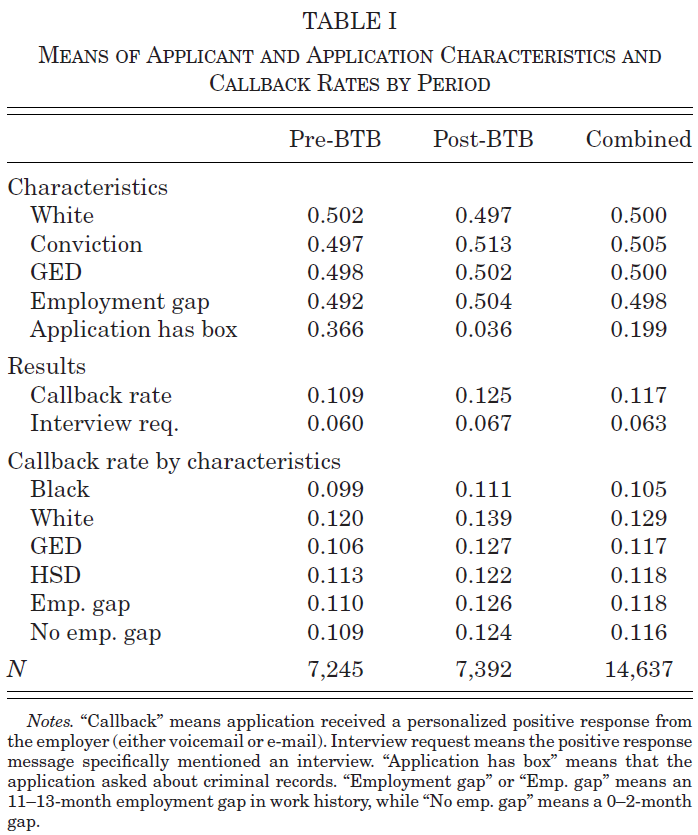
\includegraphics[scale = .6]{0925tanji/T1}
        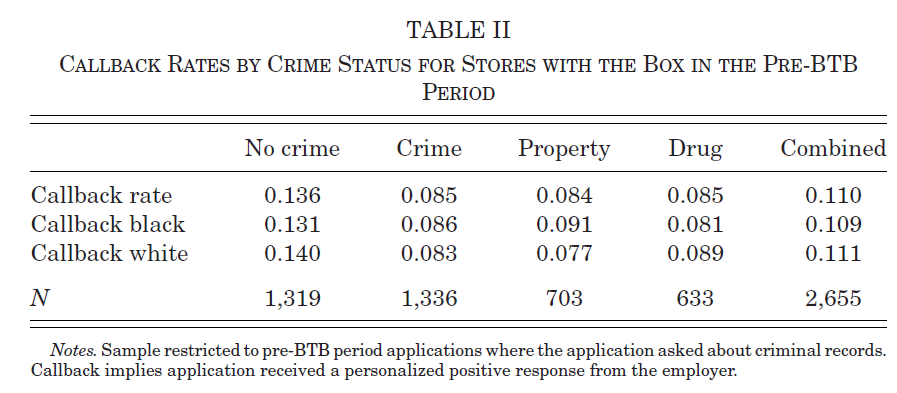
\includegraphics[scale = .6]{0925tanji/T2}
    \end{figure}

    \paragraph{Summary}

    \begin{itemize}
      \item Among pre-BTB appllications, 36.2\% had the box; there are small non-compliers (3.6\%) $Rightarrow$ box removers: 33\% of the sample.
      \begin{itemize}
        \item This rate is low, compared to the literature.
      \end{itemize}
      \item Table 1:
      \begin{itemize}
        \item The race gap from 2.1 percentage points to 2.8 percentage points in the postperiod.
        \item Callback rates hardly differed by GED/diploma status or employment gap.
      \end{itemize}
      \item pre-BTB period (Table 2)
      \begin{itemize}
        \item Criminal records does matter: callback rates were 60\% higher for applicants than those with records.
        \item Types of records does not seem to be important.
        \item Racial difference in advantage for those without records is a slight one.
      \end{itemize}
    \end{itemize}

    \paragraph{Main Effects}

    \begin{figure}[ht]
        \centering
        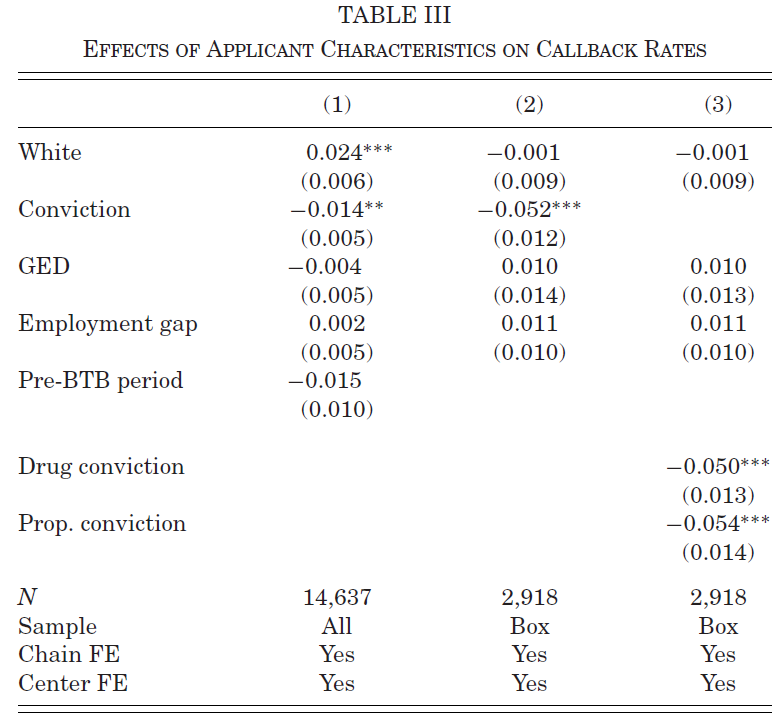
\includegraphics[scale = .6]{0925tanji/T3}
    \end{figure}

    \begin{itemize}
      \item Regression estimates:
      \begin{itemize}
        \item Baseline callback rate: 8.2\%.
        \item "white" effect is 23\% (column 1).
        \item Criminal record effect is 63\%.
      \end{itemize}
      \item (Appendix): geographic-specific effects: "white" effects is far larger in New Jersey (4.5 \% points or 8\%), while criminal record effects is larger in NY.
    \end{itemize}


    \section{The Criminal Record Box and Racial Discrimination}

    \begin{itemize}
      \item DID analyses to see the effect of criminal record information on racial discrimination.
      \item Two different sources in whether employers have the box.
      \begin{enumerate}
        \item Cross-sectional variation
        \item Temporal change after BTB
        \item Triple-differences
      \end{enumerate}
    \end{itemize}

    \subsection{Cross-Sectional DID}

    \[
    \text{Callback}_{ij} = \alpha + \beta_1 \text{Box}_j + \beta_2 \text{White}_i + \beta_3 \text{Box} \times \text{White}_i + \Gamma \mathbf{X_i} + \epsilon_{ij}
    \]

    \begin{itemize}
      \item $i, j$: indicator for applicant $i$ for store $j$.
      \item The sample includes only pre-BTB.
    \end{itemize}

    \begin{figure}[ht]
        \centering
        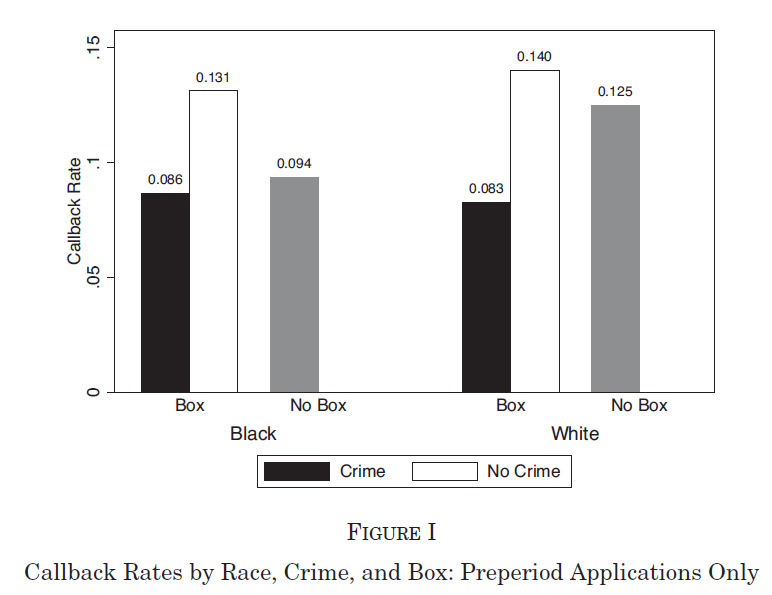
\includegraphics[scale = .8]{0925tanji/F1}
    \end{figure}

    \begin{itemize}
      \item The black-white gap is 2.8 percentage points larger among nonbox employers (p < .05) in the preperiod.
      \item Among box employers, the race gap is just .3 percentage points, while that among those without the box is ten times as large (3.1 percentage points.)

      $\Rightarrow$ Employers who lack individualized information might be relying on race-based assumptions.

      \item Two groups of employers do not vary substantially across most observable characteristics.
    \end{itemize}

    \subsection{Temporal change after BTB}

    \[
    \text{Callback}_{it} = \alpha + \beta_1 \text{White}_i + \beta_2 \text{Post}_t + \beta_3 \text{White}_i \times \text{Post}_t + \Gamma \mathbf{X_i} + \epsilon_{ij}
    \]

    \begin{itemize}
      \item $t$ indicates before/after BTB went into effect.
      \item The sample is limited to the box-remover stores (compliers).
    \end{itemize}

    \begin{figure}[ht]
        \centering
        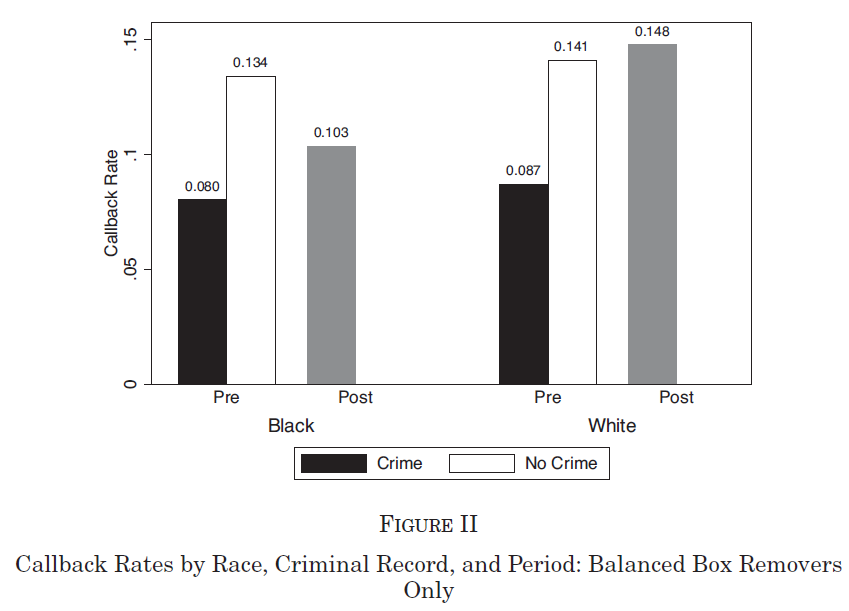
\includegraphics[scale = .8]{0925tanji/F2}
    \end{figure}

    \begin{itemize}
      \item The race gap was 3.6 percentage points smaller than after it removed, conditional on that the employer had the box before BTB.
      \item In the post-BTB period, the white callback rate was 4.4 percentage points (43\%) higher than the black baseline of 10.3\%.
      \item Notification:
      \begin{itemize}
        \item The temporal DID is more causally rigorous than the cross-sectional comparison.
        \item No-box group does not change after BTB into effect.
      \end{itemize}
    \end{itemize}

    \begin{figure}[ht]
        \centering
        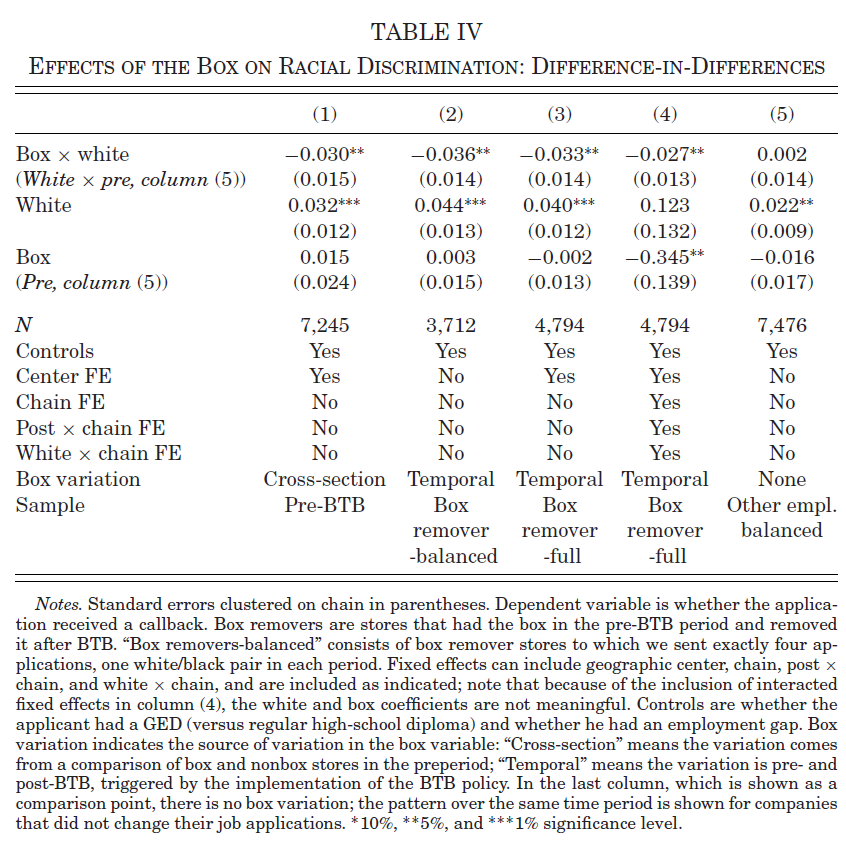
\includegraphics[scale = .8]{0925tanji/T4}
    \end{figure}

    \subsection{Triple-differences}

    \begin{itemize}
      \item To difference out the effect of any non-BTB tempral differences and control for unobserved differences between the employers.
    \end{itemize}

    \begin{align*}
      \text{Callback}_{ijt} =& \alpha + \beta_1 \text{White}_i + \beta_2 \text{Post}_t + \beta_3 \text{BoxRemover}_j \\
      & + \beta_4 \text{White}_i \times \text{Post}_t + \beta_5 \text{White}_i \times \text{BoxRemover}_j + \beta_6 \text{Post}_t \times \text{BoxRemover}_j \\
      & + \beta_7 \text{BoxRemover}_j \times \text{White}_i \times \text{Post}_t + \Gamma \mathbf{X_i} + \epsilon_{ij}
    \end{align*}

    \begin{itemize}
      \item The effect of the interest is $\beta_7$: the employer callback gap for whites versus blacks changes differently after BTB for box-remover versus other stores.
      \begin{itemize}
        \item The effect size is about 3.5 or 4.0 percentage points: the white callback rate advantage over identical black applicants grew by 3.9 percentage points after BTB.
      \end{itemize}
      \item BTB increases racial discrimination in callback rates: race gap at box-remover stores goes from .7 percentage points before BTB to 4.7 points after.
    \end{itemize}

    \begin{figure}[ht]
        \centering
        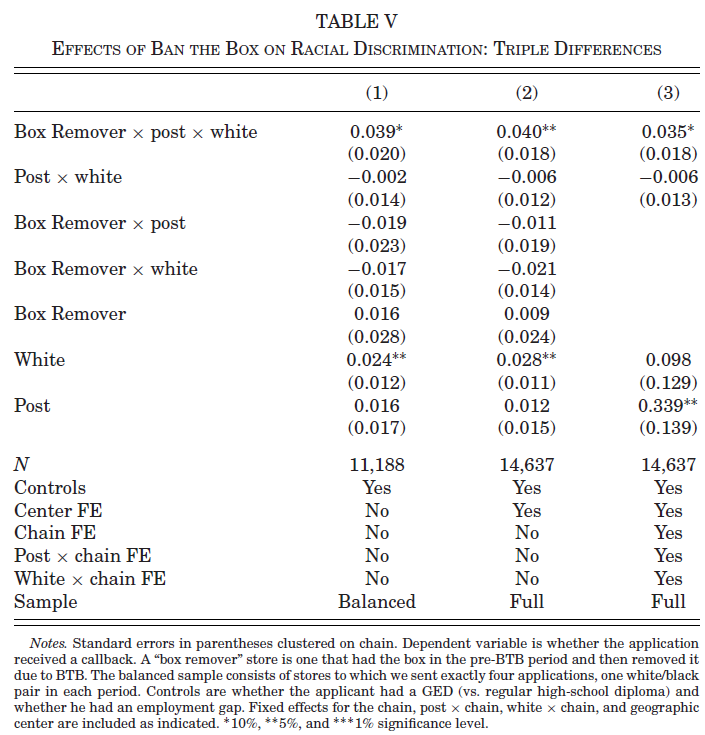
\includegraphics[scale = .8]{0925tanji/T5}
    \end{figure}

    \begin{itemize}
      \item The triple-differences approach comes at a cost in statistical power.
      \item Preperiod trends: the job applications are standardized nationally at the chain level: whether to include the box is decided at the chain level, and whether to call back is responsible for the store managers.
    \end{itemize}

    \subsection{Alternative Specifications and Smaples}

    \begin{itemize}
      \item Robustness check.
      \begin{figure}[ht]
          \centering
          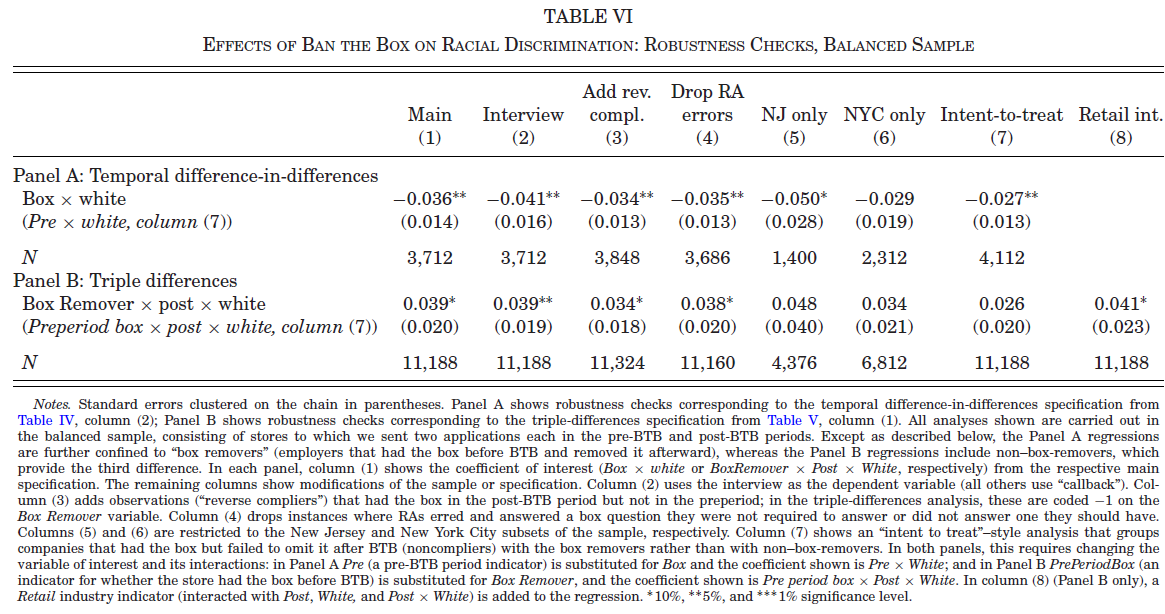
\includegraphics[scale = .8]{0925tanji/T6}
      \end{figure}
    \end{itemize}

    \section{Discussion}

    \paragraph{Who Gains and Losses from BTB?}

    \begin{itemize}
      \item BTB's basic premise: having a record poses an obastacle to employment.
      \begin{itemize}
        \item Applicants without records receive 62\% more callbacks.
        \item Even a minor, nonviolent conviction can prevent him from employment.
        \item Consitent with prior auditing studies (Pager 2003; Bonikowski, and Western 2009).
        \item It could be mitigated by BTB.
      \end{itemize}
      \item However, BTB, on the other hand, increase racial discrimination.
      \begin{itemize}
        \item The black-white gap increased sixfold (from 7\% to 43\% in callbacks).
      \end{itemize}
      \item The negative impact appears to fall on black applicants without records.
      \begin{itemize}
        \item The overall callback rates increased at least this time period.
      \end{itemize}
    \end{itemize}

    \paragraph{Mechanisms: Statistical Discrimination versus Stereotyping}

    \begin{itemize}
      \item Do employers make assumptions about balck applicants' likely criminal records?
      \begin{itemize}
        \item Most Americans subcousciously associate blackness an criminality (Eberhardt et al. 2004; Nosek et al. 2007)
        \item Bordalo et al. (2016): "kernel of the truth," or representative heuristics may exaggerate the predicted conviction rate.
      \end{itemize}
      \item National Longtitudinal Survey of Youth 1997 (NLSY97):
      \begin{itemize}
        \item The difference in self-reported conviction rate between non-Hispanic white and black males is small, which disappears entirely once differences in educational attainment are accounted.
        \item The survey does not distinguish felony convictions, which greatly differs by race (Shannon et al. 2011; Bucknor and Barber 2016).
      \end{itemize}
      \item A simple model of employers' decision making
      \[
      \text{P}(\text{call}_{ij} | \text{black}_i, \text{no box}_j) = g_b \text{P}(\text{black}_i, \text{crime}_i) + (1 - g_b) \text{P}(\text{call}_{ij} | \text{black}_i, \text{no crime}_i).
      \]
      \begin{itemize}
        \item $g_b$: the employer estimate of the probability that a black applicant has a criminal record.
        \item Using Figure 2 we can back out $g_b = 87\%$ and $g_w = 16\%$: sharply exaggerated evan relative to the largest estimates of the literature (32\%).
      \end{itemize}
      \item Other possible heuristics to make a prediction: educational status or work experience.
      \item In short, the pattern observed here is most consistent with a stereotyping model.
    \end{itemize}

    \paragraph{Identification Challenges and Limitations}

    \begin{itemize}
      \item Identification challenges
      \begin{itemize}
        \item The remaining identification threats: unobservable differences that
        \begin{itemize}
          \item affect box-remover vs. other businesses differenetly,
          \item in ways that differ by race
          \item differ time periods as well
        \end{itemize}
        \item A potential concern is that BTB might encourage real-world applicants with records to apply to box-remover companies.
      \end{itemize}
      \item Limitations
      \begin{itemize}
        \item Sample applicants were only black and white men.
        \item Focused on chain employers in the retail and restaurants.
        \item Effect on ultimate hiring pattern, instead of callbacks.
        \begin{itemize}
          \item Doleac and Hansen (2016): reduced employment of young black men in jurisdictions that adopt BTB.
        \end{itemize}
      \end{itemize}
    \end{itemize}


    \section{Conclusion}

    \begin{itemize}
      \item Their field experiment shows that employers substantially increase discrimination.
      \item 'Racial disparity is not the only policy consideration surrounding BTB, and policy makers could seek to prioritize opportunities for people with records in spite of BTB's unintended racial consequences or to mitigate those consequences in other ways. But to the extent that advocates hope that BTB itself will reduce racial disparity in employment, that hope appears misguided.'
    \end{itemize}





    %\begin{figure}[]
    %    \centering
    %    \includegraphics{template/ignore file.txt}
    %    \caption{}
    %    \label{}
    %\end{figure}

    \biblio

\end{document}
